\chapter*{前言}
\addcontentsline{toc}{chapter}{\nameref{preface}} 

引力乃人尽皆知,自我们蹒跚学步便相伴。纵使物体因它下坠,仍有许多驾驭引力的高手,如轻松掷筐的篮球球员,亦或挥拍自如的羽毛球手。鸟天生长有一对契合空气动力学的翼膀,高耸入云,更胜一筹。而大气的压强分布仍需借引力来稳定,故结论稍显意外:引力虽可能使鸟丧命,但也正是引力使鸟脱身。这皆拜引力所赐。

它如此普遍,人们自古以来便在思索其缘由。
古希腊先贤 Aristotle 认为,物体含有一定比例的重质(gravitas)和轻质(levitas),其自然运动分别向着和远离宇宙中心,但未明确动体速度与其重轻质、所处介质等的具体关系。
6 世纪,拜占庭哲学家 Philoponus 提出,任何物体于同一点皆以相同方式自由落体(free fall)。
16 世纪,意大利弥漫着复兴之息,Galileo 利用斜坡和单摆实验发现下落距离正比于时间平方,依连续性思想并忽略阻力,合理外推至自由落体。通过微积分的思想雏形,Galileo 认为任何物体于同一点加速度一致,与其质量无关。
17 世纪,人们已普遍承认 Kepler 三大定律\footnote{较早的英语文献会给人名添后缀(常为 -an)表示形容词和名词,如 Galilean, Newtonian, Jacobian。这些表达沿用至今,但对当代人物来说一般不再采取。为迎合时代,本书中这些旧时人物亦不添后缀。}:椭圆轨道、掠面恒速、周期关系。
由此 Newton 阐明了更为精确且统一天地的规律:
行星绕恒星的掠面恒速说明角动量守恒,行星所受(由 Newton 第二定律定义)的引力是有心力,必然是保守力。进而椭圆轨道现象就可将引力大小确定到平方反比距离。
用今日的术语讲,质量密度 $\mu(\bm x,t)$ 所激发的引力势 $\phi(\bm x,t)$(取无穷远为零势)满足
\[\phi(\bm x,t)=-G\int\frac{\mu(\bm x',t)}{|\bm x-\bm x'|}\,\d[3]x'\implies \nabla^2\phi(\bm x,t)=4\pi G \mu(\bm x,t).\]
此为\textbf{引力 Poisson 方程},推导类似于电场 Gauss 定律。试验质点的运动方程为 $\ddot{\bm x}=-\grad\phi$。

这一理论取得了巨大成功,但临近 20 世纪时遇到了一系列困难。
Newton 引力明显是超距的:$\bm x$ 处 $t$ 时的 $\phi$ 由空间各点一齐于 $t$ 时的 $\mu$ 决定,引力场传播无限快。而电磁学中 Coulomb 定律仅是静态解,电势应记作 $\varphi(\bm x)$。电磁学能排除超距解,因为还有涉及磁场、时间的方程参与约束。Newton 引力场论没有这种外援,因为默认平方反比律在动态也成立。Newton 尝云,\textit{平方反比律只是数学上的方便描述},但也难以提供更合理的解释了。欲解决超距作用,一种思想是想象周遭弥漫着媒介性质的物质,用于传递相互作用,即所谓\textbf{定域场},从而将平方反比作为近似情形。这一概念最初由 18 世纪 Faraday 提出,经由 Gauss、Maxwell 等人对数学的发展,定域场逐渐作为一种物理实质而占据一席。

目前实验范围内,描述引力最成功的定域场论仍归于 Albert Einstein。他另辟蹊径,于 1915 年 11 月完成了其 8 年奋斗之终幕:
\begin{figure}[ht]
    \centering
    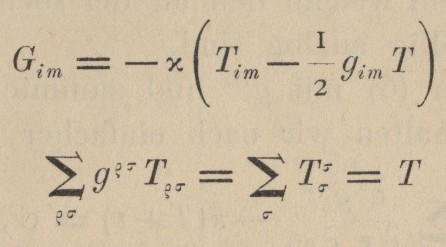
\includegraphics[scale=0.3]{fig/equation.jpeg}
    \caption*{\small 图:取自《引力的场方程》(\textit{Die Feldgleichungen der Gravitation})}
\end{figure}

\noindent Einstein 称之\textbf{广义相对论}(general relativity)。1919 年,Eddington 日全食实验验证了光线曲折的关键结论。彼时欧洲正值战后阴霾,故实验结果被相继刊登在各大报章的头版,冠之“科学革命”。这的确是现代物理学的伟大胜利。
\begin{figure}[ht]
    \centering
    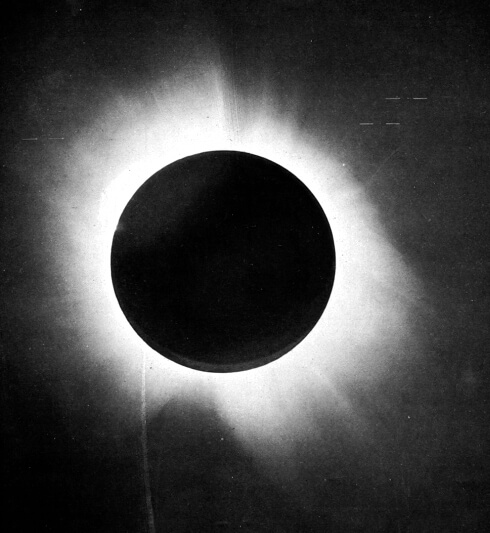
\includegraphics[scale=0.35]{fig/1919_eclipse_positive.jpg}
    \caption*{\small 图:Eddington 日全食实验结果}
\end{figure}
诚然,新符号自带神秘面纱,固然令人费解,败坏了大众印象。但我们不必妄自菲薄,无非是 Newton 理论需要微积分,而 Einstein 理论需要额外的几何学罢了。Einstein 方程仍类似于引力正比于物质的形式。它们都是人类漫漫长征的里程碑。所需的基本知识并非完全陌生,甚至一旦接受后,将发现 Einstein 的思想其实更自然、更简单。

想真正了解一套理论,仅仅知道方程还远不够。广义相对论与 20 世纪物理学所作的一些最蔚为奇观的预言相联系。读者多少在科普或艺术作品中,听说过这些现象:黑洞视界、平行宇宙、虫洞、宇宙膨胀、暗物质、信息熵、全息投影……1915 年时,这些还远未为人知,唯有人们理解方程的动力学后才能发现。花费的时间长得惊人,这其中的艰辛事迹并不逊色于 Einstein 的孤勇奋斗。本书聊物理时亦将对历史简要一瞥。目前,物理学能分析的一般解往往只是简单解的微扰,所谓的宇宙监督假设、一般条件的奇点等问题都未得到普适解答。这些问题恰恰是一套理论意义和适用范围的基础考量。我们只能期望后续理论,继续揭示出美丽的结构,帮助人类进一步认识世界。

谨以此段阐明本书之深度、广度。
本书以理工类专业一年级的多元微积分、线性代数、普通物理学为基础,致力讲述引力、时空等话题,为理解前沿进展作准备。将尽可能刨析概念动机,搭建同旧知识之桥梁。本书划分为广义相对论、数值计算以及量子理论,附录提供数学知识以飨读者。仅为证明单个命题所需的知识也放于附录,供有兴趣的读者查阅。细节未必完整提供,未提供时将给出简介和参考资料。故最终,附录在深度上似乎要讲透现代微分几何,但广度上又不完整。此乃笔者故意为之。因为本书不是要向读者大肆摆弄概念,而是补充看懂前沿所最少必要的、作了严格定义的数学。
本书看似未设习题,但实际上巧置省略,足当练习。
给出概念、结论时或通过字体改变暗示,或带编号地引入。不都采用编号只是为行文流畅,以免让本就不易的内容雪上加霜,但代价是失去链接便利。这固然重要,因为定义、命题在文中一般只出现一次,难免要来回翻阅,故敬请读者不厌其烦。

\begin{flushright}
\textit{夏草}\\
\textit{\the\year 年 \the\month 月}
\end{flushright}
\label{preface}